\documentclass[1p]{elsarticle_modified}
%\bibliographystyle{elsarticle-num}

%\usepackage[colorlinks]{hyperref}
%\usepackage{abbrmath_seonhwa} %\Abb, \Ascr, \Acal ,\Abf, \Afrak
\usepackage{amsfonts}
\usepackage{amssymb}
\usepackage{amsmath}
\usepackage{amsthm}
\usepackage{scalefnt}
\usepackage{amsbsy}
\usepackage{kotex}
\usepackage{caption}
\usepackage{subfig}
\usepackage{color}
\usepackage{graphicx}
\usepackage{xcolor} %% white, black, red, green, blue, cyan, magenta, yellow
\usepackage{float}
\usepackage{setspace}
\usepackage{hyperref}

\usepackage{tikz}
\usetikzlibrary{arrows}

\usepackage{multirow}
\usepackage{array} % fixed length table
\usepackage{hhline}

%%%%%%%%%%%%%%%%%%%%%
\makeatletter
\renewcommand*\env@matrix[1][\arraystretch]{%
	\edef\arraystretch{#1}%
	\hskip -\arraycolsep
	\let\@ifnextchar\new@ifnextchar
	\array{*\c@MaxMatrixCols c}}
\makeatother %https://tex.stackexchange.com/questions/14071/how-can-i-increase-the-line-spacing-in-a-matrix
%%%%%%%%%%%%%%%

\usepackage[normalem]{ulem}

\newcommand{\msout}[1]{\ifmmode\text{\sout{\ensuremath{#1}}}\else\sout{#1}\fi}
%SOURCE: \msout is \stkout macro in https://tex.stackexchange.com/questions/20609/strikeout-in-math-mode

\newcommand{\cancel}[1]{
	\ifmmode
	{\color{red}\msout{#1}}
	\else
	{\color{red}\sout{#1}}
	\fi
}

\newcommand{\add}[1]{
	{\color{blue}\uwave{#1}}
}

\newcommand{\replace}[2]{
	\ifmmode
	{\color{red}\msout{#1}}{\color{blue}\uwave{#2}}
	\else
	{\color{red}\sout{#1}}{\color{blue}\uwave{#2}}
	\fi
}

\newcommand{\Sol}{\mathcal{S}} %segment
\newcommand{\D}{D} %diagram
\newcommand{\A}{\mathcal{A}} %arc


%%%%%%%%%%%%%%%%%%%%%%%%%%%%%5 test

\def\sl{\operatorname{\textup{SL}}(2,\Cbb)}
\def\psl{\operatorname{\textup{PSL}}(2,\Cbb)}
\def\quan{\mkern 1mu \triangleright \mkern 1mu}

\theoremstyle{definition}
\newtheorem{thm}{Theorem}[section]
\newtheorem{prop}[thm]{Proposition}
\newtheorem{lem}[thm]{Lemma}
\newtheorem{ques}[thm]{Question}
\newtheorem{cor}[thm]{Corollary}
\newtheorem{defn}[thm]{Definition}
\newtheorem{exam}[thm]{Example}
\newtheorem{rmk}[thm]{Remark}
\newtheorem{alg}[thm]{Algorithm}

\newcommand{\I}{\sqrt{-1}}
\begin{document}

%\begin{frontmatter}
%
%\title{Boundary parabolic representations of knots up to 8 crossings}
%
%%% Group authors per affiliation:
%\author{Yunhi Cho} 
%\address{Department of Mathematics, University of Seoul, Seoul, Korea}
%\ead{yhcho@uos.ac.kr}
%
%
%\author{Seonhwa Kim} %\fnref{s_kim}}
%\address{Center for Geometry and Physics, Institute for Basic Science, Pohang, 37673, Korea}
%\ead{ryeona17@ibs.re.kr}
%
%\author{Hyuk Kim}
%\address{Department of Mathematical Sciences, Seoul National University, Seoul 08826, Korea}
%\ead{hyukkim@snu.ac.kr}
%
%\author{Seokbeom Yoon}
%\address{Department of Mathematical Sciences, Seoul National University, Seoul, 08826,  Korea}
%\ead{sbyoon15@snu.ac.kr}
%
%\begin{abstract}
%We find all boundary parabolic representation of knots up to 8 crossings.
%
%\end{abstract}
%\begin{keyword}
%    \MSC[2010] 57M25 
%\end{keyword}
%
%\end{frontmatter}

%\linenumbers
%\tableofcontents
%
\newcommand\colored[1]{\textcolor{white}{\rule[-0.35ex]{0.8em}{1.4ex}}\kern-0.8em\color{red} #1}%
%\newcommand\colored[1]{\textcolor{white}{ #1}\kern-2.17ex	\textcolor{white}{ #1}\kern-1.81ex	\textcolor{white}{ #1}\kern-2.15ex\color{red}#1	}

{\Large $\underline{12a_{0641}~(K12a_{0641})}$}

\setlength{\tabcolsep}{10pt}
\renewcommand{\arraystretch}{1.6}
\vspace{1cm}\begin{tabular}{m{100pt}>{\centering\arraybackslash}m{274pt}}
\multirow{5}{120pt}{
	\centering
	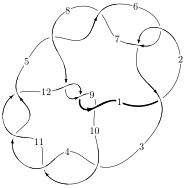
\includegraphics[width=112pt]{../../../GIT/diagram.site/Diagrams/png/1442_12a_0641.png}\\
\ \ \ A knot diagram\footnotemark}&
\allowdisplaybreaks
\textbf{Linearized knot diagam} \\
\cline{2-2}
 &
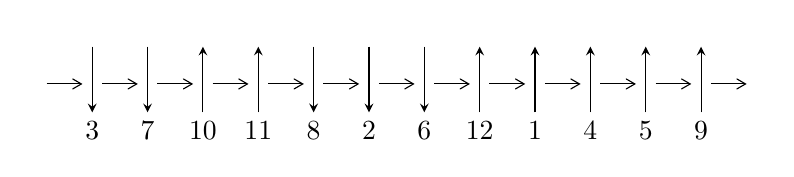
\begin{tikzpicture}[x=20pt, y=17pt]
	% nodes
	\node (C0) at (0, 0) {};
	\node (C1) at (1, 0) {};
	\node (C1U) at (1, +1) {};
	\node (C1D) at (1, -1) {3};

	\node (C2) at (2, 0) {};
	\node (C2U) at (2, +1) {};
	\node (C2D) at (2, -1) {7};

	\node (C3) at (3, 0) {};
	\node (C3U) at (3, +1) {};
	\node (C3D) at (3, -1) {10};

	\node (C4) at (4, 0) {};
	\node (C4U) at (4, +1) {};
	\node (C4D) at (4, -1) {11};

	\node (C5) at (5, 0) {};
	\node (C5U) at (5, +1) {};
	\node (C5D) at (5, -1) {8};

	\node (C6) at (6, 0) {};
	\node (C6U) at (6, +1) {};
	\node (C6D) at (6, -1) {2};

	\node (C7) at (7, 0) {};
	\node (C7U) at (7, +1) {};
	\node (C7D) at (7, -1) {6};

	\node (C8) at (8, 0) {};
	\node (C8U) at (8, +1) {};
	\node (C8D) at (8, -1) {12};

	\node (C9) at (9, 0) {};
	\node (C9U) at (9, +1) {};
	\node (C9D) at (9, -1) {1};

	\node (C10) at (10, 0) {};
	\node (C10U) at (10, +1) {};
	\node (C10D) at (10, -1) {4};

	\node (C11) at (11, 0) {};
	\node (C11U) at (11, +1) {};
	\node (C11D) at (11, -1) {5};

	\node (C12) at (12, 0) {};
	\node (C12U) at (12, +1) {};
	\node (C12D) at (12, -1) {9};
	\node (C13) at (13, 0) {};

	% arrows
	\draw[->,>={angle 60}]
	(C0) edge (C1) (C1) edge (C2) (C2) edge (C3) (C3) edge (C4) (C4) edge (C5) (C5) edge (C6) (C6) edge (C7) (C7) edge (C8) (C8) edge (C9) (C9) edge (C10) (C10) edge (C11) (C11) edge (C12) (C12) edge (C13) ;	\draw[->,>=stealth]
	(C1U) edge (C1D) (C2U) edge (C2D) (C3D) edge (C3U) (C4D) edge (C4U) (C5U) edge (C5D) (C6U) edge (C6D) (C7U) edge (C7D) (C8D) edge (C8U) (C9D) edge (C9U) (C10D) edge (C10U) (C11D) edge (C11U) (C12D) edge (C12U) ;
	\end{tikzpicture} \\
\hhline{~~} \\& 
\textbf{Solving Sequence} \\ \cline{2-2} 
 &
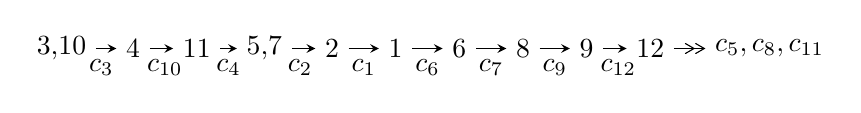
\begin{tikzpicture}[x=23pt, y=7pt]
	% node
	\node (A0) at (-1/8, 0) {3,10};
	\node (A1) at (1, 0) {4};
	\node (A2) at (2, 0) {11};
	\node (A3) at (49/16, 0) {5,7};
	\node (A4) at (33/8, 0) {2};
	\node (A5) at (41/8, 0) {1};
	\node (A6) at (49/8, 0) {6};
	\node (A7) at (57/8, 0) {8};
	\node (A8) at (65/8, 0) {9};
	\node (A9) at (73/8, 0) {12};
	\node (C1) at (1/2, -1) {$c_{3}$};
	\node (C2) at (3/2, -1) {$c_{10}$};
	\node (C3) at (5/2, -1) {$c_{4}$};
	\node (C4) at (29/8, -1) {$c_{2}$};
	\node (C5) at (37/8, -1) {$c_{1}$};
	\node (C6) at (45/8, -1) {$c_{6}$};
	\node (C7) at (53/8, -1) {$c_{7}$};
	\node (C8) at (61/8, -1) {$c_{9}$};
	\node (C9) at (69/8, -1) {$c_{12}$};
	\node (A10) at (11, 0) {$c_{5},c_{8},c_{11}$};

	% edge
	\draw[->,>=stealth]	
	(A0) edge (A1) (A1) edge (A2) (A2) edge (A3) (A3) edge (A4) (A4) edge (A5) (A5) edge (A6) (A6) edge (A7) (A7) edge (A8) (A8) edge (A9) ;
	\draw[->>,>={angle 60}]	
	(A9) edge (A10);
\end{tikzpicture} \\ 

\end{tabular} \\

\footnotetext{
The image of knot diagram is generated by the software ``\textbf{Draw programme}" developed by Andrew Bartholomew(\url{http://www.layer8.co.uk/maths/draw/index.htm\#Running-draw}), where we modified some parts for our purpose(\url{https://github.com/CATsTAILs/LinksPainter}).
}\phantom \\ \newline 
\centering \textbf{Ideals for irreducible components\footnotemark of $X_{\text{par}}$} 
 
\begin{align*}
I^u_{1}&=\langle 
9.53641\times10^{31} u^{44}+1.44960\times10^{32} u^{43}+\cdots+2.63520\times10^{32} b+1.44504\times10^{33},\\
\phantom{I^u_{1}}&\phantom{= \langle  }-9.27193\times10^{31} u^{44}-1.41274\times10^{32} u^{43}+\cdots+8.78400\times10^{31} a-1.73256\times10^{33},\;u^{45}+u^{44}+\cdots+24 u-8\rangle \\
I^u_{2}&=\langle 
2 a^2-2 a u+5 b+4 a+1,\;4 a^3+4 a^2+2 a u+6 a+7 u+8,\;u^2-2\rangle \\
\\
I^v_{1}&=\langle 
a,\;b- v+1,\;v^3-2 v^2+v-1\rangle \\
\end{align*}
\raggedright * 3 irreducible components of $\dim_{\mathbb{C}}=0$, with total 54 representations.\\
\footnotetext{All coefficients of polynomials are rational numbers. But the coefficients are sometimes approximated in decimal forms when there is not enough margin.}
\newpage
\renewcommand{\arraystretch}{1}
\centering \section*{I. $I^u_{1}= \langle 9.54\times10^{31} u^{44}+1.45\times10^{32} u^{43}+\cdots+2.64\times10^{32} b+1.45\times10^{33},\;-9.27\times10^{31} u^{44}-1.41\times10^{32} u^{43}+\cdots+8.78\times10^{31} a-1.73\times10^{33},\;u^{45}+u^{44}+\cdots+24 u-8 \rangle$}
\flushleft \textbf{(i) Arc colorings}\\
\begin{tabular}{m{7pt} m{180pt} m{7pt} m{180pt} }
\flushright $a_{3}=$&$\begin{pmatrix}1\\0\end{pmatrix}$ \\
\flushright $a_{10}=$&$\begin{pmatrix}0\\u\end{pmatrix}$ \\
\flushright $a_{4}=$&$\begin{pmatrix}1\\- u^2\end{pmatrix}$ \\
\flushright $a_{11}=$&$\begin{pmatrix}u\\- u^3+u\end{pmatrix}$ \\
\flushright $a_{5}=$&$\begin{pmatrix}- u^2+1\\u^4-2 u^2\end{pmatrix}$ \\
\flushright $a_{7}=$&$\begin{pmatrix}1.05555 u^{44}+1.60831 u^{43}+\cdots-15.1462 u+19.7241\\-0.361886 u^{44}-0.550090 u^{43}+\cdots+5.74395 u-5.48362\end{pmatrix}$ \\
\flushright $a_{2}=$&$\begin{pmatrix}0.930140 u^{44}+1.39744 u^{43}+\cdots-12.0451 u+15.7417\\-0.248255 u^{44}-0.328783 u^{43}+\cdots+4.52710 u-4.10460\end{pmatrix}$ \\
\flushright $a_{1}=$&$\begin{pmatrix}0.681885 u^{44}+1.06866 u^{43}+\cdots-7.51802 u+11.6371\\-0.248255 u^{44}-0.328783 u^{43}+\cdots+4.52710 u-4.10460\end{pmatrix}$ \\
\flushright $a_{6}=$&$\begin{pmatrix}0.373014 u^{44}+0.560645 u^{43}+\cdots-4.80141 u+7.41655\\-0.155977 u^{44}-0.247269 u^{43}+\cdots+2.81501 u-2.80465\end{pmatrix}$ \\
\flushright $a_{8}=$&$\begin{pmatrix}0.927559 u^{44}+1.36065 u^{43}+\cdots-12.7981 u+16.1079\\-0.251660 u^{44}-0.353713 u^{43}+\cdots+2.22074 u-3.09854\end{pmatrix}$ \\
\flushright $a_{9}=$&$\begin{pmatrix}-0.580385 u^{44}-0.859482 u^{43}+\cdots+7.87529 u-11.2692\\0.248579 u^{44}+0.372464 u^{43}+\cdots-2.39760 u+3.61110\end{pmatrix}$ \\
\flushright $a_{12}=$&$\begin{pmatrix}- u^3+2 u\\u^5-3 u^3+u\end{pmatrix}$\\&\end{tabular}
\flushleft \textbf{(ii) Obstruction class $= -1$}\\~\\
\flushleft \textbf{(iii) Cusp Shapes $= 0.877910 u^{44}+1.34478 u^{43}+\cdots-1.37878 u+23.3266$}\\~\\
\newpage\renewcommand{\arraystretch}{1}
\flushleft \textbf{(iv) u-Polynomials at the component}\newline \\
\begin{tabular}{m{50pt}|m{274pt}}
Crossings & \hspace{64pt}u-Polynomials at each crossing \\
\hline $$\begin{aligned}c_{1},c_{5},c_{7}\end{aligned}$$&$\begin{aligned}
&u^{45}+10 u^{44}+\cdots+36 u+1
\end{aligned}$\\
\hline $$\begin{aligned}c_{2},c_{6}\end{aligned}$$&$\begin{aligned}
&u^{45}-2 u^{44}+\cdots-8 u+1
\end{aligned}$\\
\hline $$\begin{aligned}c_{3},c_{4},c_{10}\\c_{11}\end{aligned}$$&$\begin{aligned}
&u^{45}+u^{44}+\cdots+24 u-8
\end{aligned}$\\
\hline $$\begin{aligned}c_{8},c_{9},c_{12}\end{aligned}$$&$\begin{aligned}
&u^{45}-4 u^{44}+\cdots+69 u+23
\end{aligned}$\\
\hline
\end{tabular}\\~\\
\newpage\renewcommand{\arraystretch}{1}
\flushleft \textbf{(v) Riley Polynomials at the component}\newline \\
\begin{tabular}{m{50pt}|m{274pt}}
Crossings & \hspace{64pt}Riley Polynomials at each crossing \\
\hline $$\begin{aligned}c_{1},c_{5},c_{7}\end{aligned}$$&$\begin{aligned}
&y^{45}+54 y^{44}+\cdots+420 y-1
\end{aligned}$\\
\hline $$\begin{aligned}c_{2},c_{6}\end{aligned}$$&$\begin{aligned}
&y^{45}-10 y^{44}+\cdots+36 y-1
\end{aligned}$\\
\hline $$\begin{aligned}c_{3},c_{4},c_{10}\\c_{11}\end{aligned}$$&$\begin{aligned}
&y^{45}-59 y^{44}+\cdots+576 y-64
\end{aligned}$\\
\hline $$\begin{aligned}c_{8},c_{9},c_{12}\end{aligned}$$&$\begin{aligned}
&y^{45}-52 y^{44}+\cdots+5635 y-529
\end{aligned}$\\
\hline
\end{tabular}\\~\\
\newpage\flushleft \textbf{(vi) Complex Volumes and Cusp Shapes}
$$\begin{array}{c|c|c}  
\text{Solutions to }I^u_{1}& \I (\text{vol} + \sqrt{-1}CS) & \text{Cusp shape}\\
 \hline 
\begin{aligned}
u &= -0.926963 + 0.277106 I \\
a &= -0.09767 - 2.10895 I \\
b &= \phantom{-}0.912053 + 0.832400 I\end{aligned}
 & \phantom{-}6.86189 - 5.36898 I & \phantom{-}8.49956 + 6.61909 I \\ \hline\begin{aligned}
u &= -0.926963 - 0.277106 I \\
a &= -0.09767 + 2.10895 I \\
b &= \phantom{-}0.912053 - 0.832400 I\end{aligned}
 & \phantom{-}6.86189 + 5.36898 I & \phantom{-}8.49956 - 6.61909 I \\ \hline\begin{aligned}
u &= \phantom{-}0.941670 + 0.205124 I \\
a &= -1.03689 - 1.25346 I \\
b &= \phantom{-}0.891051 + 0.833627 I\end{aligned}
 & \phantom{-}6.92054 - 0.83550 I & \phantom{-}8.82992 - 1.28747 I \\ \hline\begin{aligned}
u &= \phantom{-}0.941670 - 0.205124 I \\
a &= -1.03689 + 1.25346 I \\
b &= \phantom{-}0.891051 - 0.833627 I\end{aligned}
 & \phantom{-}6.92054 + 0.83550 I & \phantom{-}8.82992 + 1.28747 I \\ \hline\begin{aligned}
u &= \phantom{-}0.023683 + 0.934020 I \\
a &= -0.543202 + 0.459579 I \\
b &= -0.929182 - 0.891513 I\end{aligned}
 & \phantom{-}11.64400 - 3.29131 I & \phantom{-}8.32249 + 2.32768 I \\ \hline\begin{aligned}
u &= \phantom{-}0.023683 - 0.934020 I \\
a &= -0.543202 - 0.459579 I \\
b &= -0.929182 + 0.891513 I\end{aligned}
 & \phantom{-}11.64400 + 3.29131 I & \phantom{-}8.32249 - 2.32768 I \\ \hline\begin{aligned}
u &= \phantom{-}0.846105 + 0.378892 I \\
a &= -1.22689 - 1.16468 I \\
b &= -0.954555 + 0.513401 I\end{aligned}
 & \phantom{-}5.23947 + 5.34835 I & \phantom{-}7.95547 - 7.29971 I \\ \hline\begin{aligned}
u &= \phantom{-}0.846105 - 0.378892 I \\
a &= -1.22689 + 1.16468 I \\
b &= -0.954555 - 0.513401 I\end{aligned}
 & \phantom{-}5.23947 - 5.34835 I & \phantom{-}7.95547 + 7.29971 I \\ \hline\begin{aligned}
u &= -1.039870 + 0.275140 I \\
a &= \phantom{-}0.288564 - 0.168386 I \\
b &= -0.452638 + 0.664033 I\end{aligned}
 & \phantom{-}6.82014 - 0.93085 I & \phantom{-}11.70994 + 0.69834 I \\ \hline\begin{aligned}
u &= -1.039870 - 0.275140 I \\
a &= \phantom{-}0.288564 + 0.168386 I \\
b &= -0.452638 - 0.664033 I\end{aligned}
 & \phantom{-}6.82014 + 0.93085 I & \phantom{-}11.70994 - 0.69834 I\\
 \hline 
 \end{array}$$\newpage$$\begin{array}{c|c|c}  
\text{Solutions to }I^u_{1}& \I (\text{vol} + \sqrt{-1}CS) & \text{Cusp shape}\\
 \hline 
\begin{aligned}
u &= \phantom{-}0.966296 + 0.676286 I \\
a &= \phantom{-}0.61696 + 1.64433 I \\
b &= \phantom{-}0.973987 - 0.877117 I\end{aligned}
 & \phantom{-}14.4733 + 8.6224 I & \phantom{-0.000000 } 0 \\ \hline\begin{aligned}
u &= \phantom{-}0.966296 - 0.676286 I \\
a &= \phantom{-}0.61696 - 1.64433 I \\
b &= \phantom{-}0.973987 + 0.877117 I\end{aligned}
 & \phantom{-}14.4733 - 8.6224 I & \phantom{-0.000000 } 0 \\ \hline\begin{aligned}
u &= -1.009550 + 0.656162 I \\
a &= -0.644421 + 0.462034 I \\
b &= \phantom{-}0.886665 - 0.920023 I\end{aligned}
 & \phantom{-}14.7553 - 1.9983 I & \phantom{-0.000000 } 0 \\ \hline\begin{aligned}
u &= -1.009550 - 0.656162 I \\
a &= -0.644421 - 0.462034 I \\
b &= \phantom{-}0.886665 + 0.920023 I\end{aligned}
 & \phantom{-}14.7553 + 1.9983 I & \phantom{-0.000000 } 0 \\ \hline\begin{aligned}
u &= \phantom{-}0.790311\phantom{ +0.000000I} \\
a &= \phantom{-}1.71120\phantom{ +0.000000I} \\
b &= \phantom{-}0.978813\phantom{ +0.000000I}\end{aligned}
 & \phantom{-}2.25051\phantom{ +0.000000I} & \phantom{-}5.01630\phantom{ +0.000000I} \\ \hline\begin{aligned}
u &= -0.585865 + 0.317408 I \\
a &= -0.78884 + 1.75623 I \\
b &= -0.805345 - 0.377442 I\end{aligned}
 & -0.16293 - 3.03748 I & \phantom{-}3.07976 + 9.52409 I \\ \hline\begin{aligned}
u &= -0.585865 - 0.317408 I \\
a &= -0.78884 - 1.75623 I \\
b &= -0.805345 + 0.377442 I\end{aligned}
 & -0.16293 + 3.03748 I & \phantom{-}3.07976 - 9.52409 I \\ \hline\begin{aligned}
u &= -1.37682\phantom{ +0.000000I} \\
a &= -0.746455\phantom{ +0.000000I} \\
b &= -0.218102\phantom{ +0.000000I}\end{aligned}
 & \phantom{-}6.50761\phantom{ +0.000000I} & \phantom{-0.000000 } 0 \\ \hline\begin{aligned}
u &= \phantom{-}0.131062 + 0.586653 I \\
a &= \phantom{-}1.24295 + 0.87480 I \\
b &= \phantom{-}0.739277 + 0.534527 I\end{aligned}
 & \phantom{-}3.06266 - 2.04715 I & \phantom{-}4.85763 + 2.56353 I \\ \hline\begin{aligned}
u &= \phantom{-}0.131062 - 0.586653 I \\
a &= \phantom{-}1.24295 - 0.87480 I \\
b &= \phantom{-}0.739277 - 0.534527 I\end{aligned}
 & \phantom{-}3.06266 + 2.04715 I & \phantom{-}4.85763 - 2.56353 I\\
 \hline 
 \end{array}$$\newpage$$\begin{array}{c|c|c}  
\text{Solutions to }I^u_{1}& \I (\text{vol} + \sqrt{-1}CS) & \text{Cusp shape}\\
 \hline 
\begin{aligned}
u &= \phantom{-}1.46705\phantom{ +0.000000I} \\
a &= -0.579352\phantom{ +0.000000I} \\
b &= -0.870479\phantom{ +0.000000I}\end{aligned}
 & \phantom{-}4.13430\phantom{ +0.000000I} & \phantom{-0.000000 } 0 \\ \hline\begin{aligned}
u &= \phantom{-}0.519844 + 0.033701 I \\
a &= \phantom{-}0.914229 + 0.857221 I \\
b &= -0.417105 - 0.301945 I\end{aligned}
 & \phantom{-}0.905318 + 0.103320 I & \phantom{-}10.97546 - 0.25661 I \\ \hline\begin{aligned}
u &= \phantom{-}0.519844 - 0.033701 I \\
a &= \phantom{-}0.914229 - 0.857221 I \\
b &= -0.417105 + 0.301945 I\end{aligned}
 & \phantom{-}0.905318 - 0.103320 I & \phantom{-}10.97546 + 0.25661 I \\ \hline\begin{aligned}
u &= \phantom{-}1.54974 + 0.04851 I \\
a &= \phantom{-}0.02206 + 1.51683 I \\
b &= \phantom{-}0.884978 - 0.530874 I\end{aligned}
 & \phantom{-}7.04735 + 4.23377 I & \phantom{-0.000000 } 0 \\ \hline\begin{aligned}
u &= \phantom{-}1.54974 - 0.04851 I \\
a &= \phantom{-}0.02206 - 1.51683 I \\
b &= \phantom{-}0.884978 + 0.530874 I\end{aligned}
 & \phantom{-}7.04735 - 4.23377 I & \phantom{-0.000000 } 0 \\ \hline\begin{aligned}
u &= -1.55369 + 0.03708 I \\
a &= -0.48020 - 1.33204 I \\
b &= \phantom{-}0.578245 + 0.609458 I\end{aligned}
 & \phantom{-}8.03802 - 0.09902 I & \phantom{-0.000000 } 0 \\ \hline\begin{aligned}
u &= -1.55369 - 0.03708 I \\
a &= -0.48020 + 1.33204 I \\
b &= \phantom{-}0.578245 - 0.609458 I\end{aligned}
 & \phantom{-}8.03802 + 0.09902 I & \phantom{-0.000000 } 0 \\ \hline\begin{aligned}
u &= \phantom{-}0.001231 + 0.423155 I \\
a &= -0.622949 - 0.533249 I \\
b &= -0.883296 + 0.781171 I\end{aligned}
 & \phantom{-}3.96310 + 2.93834 I & -0.43677 - 3.36885 I \\ \hline\begin{aligned}
u &= \phantom{-}0.001231 - 0.423155 I \\
a &= -0.622949 + 0.533249 I \\
b &= -0.883296 - 0.781171 I\end{aligned}
 & \phantom{-}3.96310 - 2.93834 I & -0.43677 + 3.36885 I \\ \hline\begin{aligned}
u &= -0.208519 + 0.357357 I \\
a &= \phantom{-}1.310670 - 0.182130 I \\
b &= \phantom{-}0.753961 - 0.173670 I\end{aligned}
 & -1.242180 + 0.549575 I & -4.50079 - 0.85707 I\\
 \hline 
 \end{array}$$\newpage$$\begin{array}{c|c|c}  
\text{Solutions to }I^u_{1}& \I (\text{vol} + \sqrt{-1}CS) & \text{Cusp shape}\\
 \hline 
\begin{aligned}
u &= -0.208519 - 0.357357 I \\
a &= \phantom{-}1.310670 + 0.182130 I \\
b &= \phantom{-}0.753961 + 0.173670 I\end{aligned}
 & -1.242180 - 0.549575 I & -4.50079 + 0.85707 I \\ \hline\begin{aligned}
u &= \phantom{-}0.378626\phantom{ +0.000000I} \\
a &= \phantom{-}2.77102\phantom{ +0.000000I} \\
b &= -0.520904\phantom{ +0.000000I}\end{aligned}
 & \phantom{-}0.938924\phantom{ +0.000000I} & \phantom{-}14.9190\phantom{ +0.000000I} \\ \hline\begin{aligned}
u &= -1.67565\phantom{ +0.000000I} \\
a &= -0.581072\phantom{ +0.000000I} \\
b &= -1.13016\phantom{ +0.000000I}\end{aligned}
 & \phantom{-}11.0611\phantom{ +0.000000I} & \phantom{-0.000000 } 0 \\ \hline\begin{aligned}
u &= -1.68688 + 0.09794 I \\
a &= \phantom{-}0.373353 - 1.216300 I \\
b &= \phantom{-}1.087160 + 0.497430 I\end{aligned}
 & \phantom{-}14.1681 - 7.1706 I & \phantom{-0.000000 } 0 \\ \hline\begin{aligned}
u &= -1.68688 - 0.09794 I \\
a &= \phantom{-}0.373353 + 1.216300 I \\
b &= \phantom{-}1.087160 - 0.497430 I\end{aligned}
 & \phantom{-}14.1681 + 7.1706 I & \phantom{-0.000000 } 0 \\ \hline\begin{aligned}
u &= \phantom{-}1.70518 + 0.07345 I \\
a &= \phantom{-}0.48413 - 1.95464 I \\
b &= -0.959387 + 0.884389 I\end{aligned}
 & \phantom{-}16.2110 + 6.7605 I & \phantom{-0.000000 } 0 \\ \hline\begin{aligned}
u &= \phantom{-}1.70518 - 0.07345 I \\
a &= \phantom{-}0.48413 + 1.95464 I \\
b &= -0.959387 - 0.884389 I\end{aligned}
 & \phantom{-}16.2110 - 6.7605 I & \phantom{-0.000000 } 0 \\ \hline\begin{aligned}
u &= -1.70989 + 0.04785 I \\
a &= \phantom{-}0.92219 - 1.55641 I \\
b &= -0.903637 + 0.911957 I\end{aligned}
 & \phantom{-}16.3914 - 0.1365 I & \phantom{-0.000000 } 0 \\ \hline\begin{aligned}
u &= -1.70989 - 0.04785 I \\
a &= \phantom{-}0.92219 + 1.55641 I \\
b &= -0.903637 - 0.911957 I\end{aligned}
 & \phantom{-}16.3914 + 0.1365 I & \phantom{-0.000000 } 0 \\ \hline\begin{aligned}
u &= \phantom{-}1.72676 + 0.05968 I \\
a &= -0.360921 - 0.923368 I \\
b &= \phantom{-}0.343715 + 0.875406 I\end{aligned}
 & \phantom{-}16.6790 + 2.2118 I & \phantom{-0.000000 } 0\\
 \hline 
 \end{array}$$\newpage$$\begin{array}{c|c|c}  
\text{Solutions to }I^u_{1}& \I (\text{vol} + \sqrt{-1}CS) & \text{Cusp shape}\\
 \hline 
\begin{aligned}
u &= \phantom{-}1.72676 - 0.05968 I \\
a &= -0.360921 + 0.923368 I \\
b &= \phantom{-}0.343715 - 0.875406 I\end{aligned}
 & \phantom{-}16.6790 - 2.2118 I & \phantom{-0.000000 } 0 \\ \hline\begin{aligned}
u &= -1.72249 + 0.20334 I \\
a &= -0.05274 + 1.88408 I \\
b &= -1.020410 - 0.868678 I\end{aligned}
 & -15.7769 - 12.1806 I & \phantom{-0.000000 } 0 \\ \hline\begin{aligned}
u &= -1.72249 - 0.20334 I \\
a &= -0.05274 - 1.88408 I \\
b &= -1.020410 + 0.868678 I\end{aligned}
 & -15.7769 + 12.1806 I & \phantom{-0.000000 } 0 \\ \hline\begin{aligned}
u &= \phantom{-}1.74036 + 0.18867 I \\
a &= \phantom{-}0.891945 + 1.020600 I \\
b &= -0.845114 - 0.962160 I\end{aligned}
 & -15.2052 + 5.4595 I & \phantom{-0.000000 } 0 \\ \hline\begin{aligned}
u &= \phantom{-}1.74036 - 0.18867 I \\
a &= \phantom{-}0.891945 - 1.020600 I \\
b &= -0.845114 + 0.962160 I\end{aligned}
 & -15.2052 - 5.4595 I & \phantom{-0.000000 } 0\\
 \hline 
 \end{array}$$\newpage\newpage\renewcommand{\arraystretch}{1}
\centering \section*{II. $I^u_{2}= \langle 2 a^2-2 a u+5 b+4 a+1,\;4 a^3+4 a^2+2 a u+6 a+7 u+8,\;u^2-2 \rangle$}
\flushleft \textbf{(i) Arc colorings}\\
\begin{tabular}{m{7pt} m{180pt} m{7pt} m{180pt} }
\flushright $a_{3}=$&$\begin{pmatrix}1\\0\end{pmatrix}$ \\
\flushright $a_{10}=$&$\begin{pmatrix}0\\u\end{pmatrix}$ \\
\flushright $a_{4}=$&$\begin{pmatrix}1\\-2\end{pmatrix}$ \\
\flushright $a_{11}=$&$\begin{pmatrix}u\\- u\end{pmatrix}$ \\
\flushright $a_{5}=$&$\begin{pmatrix}-1\\0\end{pmatrix}$ \\
\flushright $a_{7}=$&$\begin{pmatrix}a\\-\frac{2}{5} a^2+\frac{2}{5} a u-\frac{4}{5} a-\frac{1}{5}\end{pmatrix}$ \\
\flushright $a_{2}=$&$\begin{pmatrix}-\frac{2}{5} a^2 u-\frac{1}{5} a u+\cdots-\frac{2}{5} a+\frac{1}{5}\\\frac{2}{5} a^2 u+\frac{1}{5} a u+\cdots+\frac{2}{5} a-\frac{1}{5}\end{pmatrix}$ \\
\flushright $a_{1}=$&$\begin{pmatrix}-\frac{1}{2} u\\\frac{2}{5} a^2 u+\frac{1}{5} a u+\cdots+\frac{2}{5} a-\frac{1}{5}\end{pmatrix}$ \\
\flushright $a_{6}=$&$\begin{pmatrix}-\frac{1}{5} a^2 u+\frac{1}{5} a u+\cdots+\frac{1}{5} a-\frac{4}{5}\\\frac{2}{5} a^2 u+\frac{3}{5} a u+\cdots-\frac{2}{5} a+\frac{3}{5}\end{pmatrix}$ \\
\flushright $a_{8}=$&$\begin{pmatrix}-\frac{1}{2} u\\\frac{2}{5} a^2 u+\frac{1}{5} a u+\cdots+\frac{2}{5} a-\frac{1}{5}\end{pmatrix}$ \\
\flushright $a_{9}=$&$\begin{pmatrix}-\frac{1}{2} u\\\frac{2}{5} a^2 u+\frac{1}{5} a u+\cdots+\frac{2}{5} a-\frac{1}{5}\end{pmatrix}$ \\
\flushright $a_{12}=$&$\begin{pmatrix}0\\- u\end{pmatrix}$\\&\end{tabular}
\flushleft \textbf{(ii) Obstruction class $= 1$}\\~\\
\flushleft \textbf{(iii) Cusp Shapes $= -\frac{8}{5} a^2+\frac{8}{5} a u-\frac{16}{5} a+\frac{36}{5}$}\\~\\
\newpage\renewcommand{\arraystretch}{1}
\flushleft \textbf{(iv) u-Polynomials at the component}\newline \\
\begin{tabular}{m{50pt}|m{274pt}}
Crossings & \hspace{64pt}u-Polynomials at each crossing \\
\hline $$\begin{aligned}c_{1},c_{5}\end{aligned}$$&$\begin{aligned}
&(u^3- u^2+2 u-1)^2
\end{aligned}$\\
\hline $$\begin{aligned}c_{2}\end{aligned}$$&$\begin{aligned}
&(u^3- u^2+1)^2
\end{aligned}$\\
\hline $$\begin{aligned}c_{3},c_{4},c_{10}\\c_{11}\end{aligned}$$&$\begin{aligned}
&(u^2-2)^3
\end{aligned}$\\
\hline $$\begin{aligned}c_{6}\end{aligned}$$&$\begin{aligned}
&(u^3+u^2-1)^2
\end{aligned}$\\
\hline $$\begin{aligned}c_{7}\end{aligned}$$&$\begin{aligned}
&(u^3+u^2+2 u+1)^2
\end{aligned}$\\
\hline $$\begin{aligned}c_{8},c_{9}\end{aligned}$$&$\begin{aligned}
&(u-1)^6
\end{aligned}$\\
\hline $$\begin{aligned}c_{12}\end{aligned}$$&$\begin{aligned}
&(u+1)^6
\end{aligned}$\\
\hline
\end{tabular}\\~\\
\newpage\renewcommand{\arraystretch}{1}
\flushleft \textbf{(v) Riley Polynomials at the component}\newline \\
\begin{tabular}{m{50pt}|m{274pt}}
Crossings & \hspace{64pt}Riley Polynomials at each crossing \\
\hline $$\begin{aligned}c_{1},c_{5},c_{7}\end{aligned}$$&$\begin{aligned}
&(y^3+3 y^2+2 y-1)^2
\end{aligned}$\\
\hline $$\begin{aligned}c_{2},c_{6}\end{aligned}$$&$\begin{aligned}
&(y^3- y^2+2 y-1)^2
\end{aligned}$\\
\hline $$\begin{aligned}c_{3},c_{4},c_{10}\\c_{11}\end{aligned}$$&$\begin{aligned}
&(y-2)^6
\end{aligned}$\\
\hline $$\begin{aligned}c_{8},c_{9},c_{12}\end{aligned}$$&$\begin{aligned}
&(y-1)^6
\end{aligned}$\\
\hline
\end{tabular}\\~\\
\newpage\flushleft \textbf{(vi) Complex Volumes and Cusp Shapes}
$$\begin{array}{c|c|c}  
\text{Solutions to }I^u_{2}& \I (\text{vol} + \sqrt{-1}CS) & \text{Cusp shape}\\
 \hline 
\begin{aligned}
u &= \phantom{-}1.41421\phantom{ +0.000000I} \\
a &= -1.50656\phantom{ +0.000000I} \\
b &= -0.754878\phantom{ +0.000000I}\end{aligned}
 & \phantom{-}5.46628\phantom{ +0.000000I} & \phantom{-}4.98050\phantom{ +0.000000I} \\ \hline\begin{aligned}
u &= \phantom{-}1.41421\phantom{ +0.000000I} \\
a &= \phantom{-}0.25328 + 1.70473 I \\
b &= \phantom{-}0.877439 - 0.744862 I\end{aligned}
 & \phantom{-}9.60386 + 2.82812 I & \phantom{-}11.50976 - 2.97945 I \\ \hline\begin{aligned}
u &= \phantom{-}1.41421\phantom{ +0.000000I} \\
a &= \phantom{-}0.25328 - 1.70473 I \\
b &= \phantom{-}0.877439 + 0.744862 I\end{aligned}
 & \phantom{-}9.60386 - 2.82812 I & \phantom{-}11.50976 + 2.97945 I \\ \hline\begin{aligned}
u &= -1.41421\phantom{ +0.000000I} \\
a &= -0.683438 + 0.909550 I \\
b &= \phantom{-}0.877439 - 0.744862 I\end{aligned}
 & \phantom{-}9.60386 + 2.82812 I & \phantom{-}11.50976 - 2.97945 I \\ \hline\begin{aligned}
u &= -1.41421\phantom{ +0.000000I} \\
a &= -0.683438 - 0.909550 I \\
b &= \phantom{-}0.877439 + 0.744862 I\end{aligned}
 & \phantom{-}9.60386 - 2.82812 I & \phantom{-}11.50976 + 2.97945 I \\ \hline\begin{aligned}
u &= -1.41421\phantom{ +0.000000I} \\
a &= \phantom{-}0.366877\phantom{ +0.000000I} \\
b &= -0.754878\phantom{ +0.000000I}\end{aligned}
 & \phantom{-}5.46628\phantom{ +0.000000I} & \phantom{-}4.98050\phantom{ +0.000000I}\\
 \hline 
 \end{array}$$\newpage\newpage\renewcommand{\arraystretch}{1}
\centering \section*{III. $I^v_{1}= \langle a,\;b- v+1,\;v^3-2 v^2+v-1 \rangle$}
\flushleft \textbf{(i) Arc colorings}\\
\begin{tabular}{m{7pt} m{180pt} m{7pt} m{180pt} }
\flushright $a_{3}=$&$\begin{pmatrix}1\\0\end{pmatrix}$ \\
\flushright $a_{10}=$&$\begin{pmatrix}v\\0\end{pmatrix}$ \\
\flushright $a_{4}=$&$\begin{pmatrix}1\\0\end{pmatrix}$ \\
\flushright $a_{11}=$&$\begin{pmatrix}v\\0\end{pmatrix}$ \\
\flushright $a_{5}=$&$\begin{pmatrix}1\\0\end{pmatrix}$ \\
\flushright $a_{7}=$&$\begin{pmatrix}0\\v-1\end{pmatrix}$ \\
\flushright $a_{2}=$&$\begin{pmatrix}1\\- v^2+2 v-1\end{pmatrix}$ \\
\flushright $a_{1}=$&$\begin{pmatrix}- v^2+2 v\\- v^2+2 v-1\end{pmatrix}$ \\
\flushright $a_{6}=$&$\begin{pmatrix}v-1\\v^2- v-1\end{pmatrix}$ \\
\flushright $a_{8}=$&$\begin{pmatrix}v^2-2 v\\v^2-2 v+1\end{pmatrix}$ \\
\flushright $a_{9}=$&$\begin{pmatrix}v^2- v\\v^2-2 v+1\end{pmatrix}$ \\
\flushright $a_{12}=$&$\begin{pmatrix}v\\0\end{pmatrix}$\\&\end{tabular}
\flushleft \textbf{(ii) Obstruction class $= 1$}\\~\\
\flushleft \textbf{(iii) Cusp Shapes $= -4 v^2-2 v+10$}\\~\\
\newpage\renewcommand{\arraystretch}{1}
\flushleft \textbf{(iv) u-Polynomials at the component}\newline \\
\begin{tabular}{m{50pt}|m{274pt}}
Crossings & \hspace{64pt}u-Polynomials at each crossing \\
\hline $$\begin{aligned}c_{1},c_{5}\end{aligned}$$&$\begin{aligned}
&u^3- u^2+2 u-1
\end{aligned}$\\
\hline $$\begin{aligned}c_{2}\end{aligned}$$&$\begin{aligned}
&u^3+u^2-1
\end{aligned}$\\
\hline $$\begin{aligned}c_{3},c_{4},c_{10}\\c_{11}\end{aligned}$$&$\begin{aligned}
&u^3
\end{aligned}$\\
\hline $$\begin{aligned}c_{6}\end{aligned}$$&$\begin{aligned}
&u^3- u^2+1
\end{aligned}$\\
\hline $$\begin{aligned}c_{7}\end{aligned}$$&$\begin{aligned}
&u^3+u^2+2 u+1
\end{aligned}$\\
\hline $$\begin{aligned}c_{8},c_{9}\end{aligned}$$&$\begin{aligned}
&(u+1)^3
\end{aligned}$\\
\hline $$\begin{aligned}c_{12}\end{aligned}$$&$\begin{aligned}
&(u-1)^3
\end{aligned}$\\
\hline
\end{tabular}\\~\\
\newpage\renewcommand{\arraystretch}{1}
\flushleft \textbf{(v) Riley Polynomials at the component}\newline \\
\begin{tabular}{m{50pt}|m{274pt}}
Crossings & \hspace{64pt}Riley Polynomials at each crossing \\
\hline $$\begin{aligned}c_{1},c_{5},c_{7}\end{aligned}$$&$\begin{aligned}
&y^3+3 y^2+2 y-1
\end{aligned}$\\
\hline $$\begin{aligned}c_{2},c_{6}\end{aligned}$$&$\begin{aligned}
&y^3- y^2+2 y-1
\end{aligned}$\\
\hline $$\begin{aligned}c_{3},c_{4},c_{10}\\c_{11}\end{aligned}$$&$\begin{aligned}
&y^3
\end{aligned}$\\
\hline $$\begin{aligned}c_{8},c_{9},c_{12}\end{aligned}$$&$\begin{aligned}
&(y-1)^3
\end{aligned}$\\
\hline
\end{tabular}\\~\\
\newpage\flushleft \textbf{(vi) Complex Volumes and Cusp Shapes}
$$\begin{array}{c|c|c}  
\text{Solutions to }I^v_{1}& \I (\text{vol} + \sqrt{-1}CS) & \text{Cusp shape}\\
 \hline 
\begin{aligned}
v &= \phantom{-}0.122561 + 0.744862 I \\
a &= \phantom{-0.000000 } 0 \\
b &= -0.877439 + 0.744862 I\end{aligned}
 & \phantom{-}4.66906 + 2.82812 I & \phantom{-}11.91407 - 2.22005 I \\ \hline\begin{aligned}
v &= \phantom{-}0.122561 - 0.744862 I \\
a &= \phantom{-0.000000 } 0 \\
b &= -0.877439 - 0.744862 I\end{aligned}
 & \phantom{-}4.66906 - 2.82812 I & \phantom{-}11.91407 + 2.22005 I \\ \hline\begin{aligned}
v &= \phantom{-}1.75488\phantom{ +0.000000I} \\
a &= \phantom{-0.000000 } 0 \\
b &= \phantom{-}0.754878\phantom{ +0.000000I}\end{aligned}
 & \phantom{-}0.531480\phantom{ +0.000000I} & -5.82810\phantom{ +0.000000I}\\
 \hline 
 \end{array}$$\newpage
\newpage\renewcommand{\arraystretch}{1}
\centering \section*{ IV. u-Polynomials}
\begin{tabular}{m{50pt}|m{274pt}}
Crossings & \hspace{64pt}u-Polynomials at each crossing \\
\hline $$\begin{aligned}c_{1},c_{5}\end{aligned}$$&$\begin{aligned}
&((u^3- u^2+2 u-1)^3)(u^{45}+10 u^{44}+\cdots+36 u+1)
\end{aligned}$\\
\hline $$\begin{aligned}c_{2}\end{aligned}$$&$\begin{aligned}
&((u^3- u^2+1)^2)(u^3+u^2-1)(u^{45}-2 u^{44}+\cdots-8 u+1)
\end{aligned}$\\
\hline $$\begin{aligned}c_{3},c_{4},c_{10}\\c_{11}\end{aligned}$$&$\begin{aligned}
&u^3(u^2-2)^3(u^{45}+u^{44}+\cdots+24 u-8)
\end{aligned}$\\
\hline $$\begin{aligned}c_{6}\end{aligned}$$&$\begin{aligned}
&(u^3- u^2+1)(u^3+u^2-1)^2(u^{45}-2 u^{44}+\cdots-8 u+1)
\end{aligned}$\\
\hline $$\begin{aligned}c_{7}\end{aligned}$$&$\begin{aligned}
&((u^3+u^2+2 u+1)^3)(u^{45}+10 u^{44}+\cdots+36 u+1)
\end{aligned}$\\
\hline $$\begin{aligned}c_{8},c_{9}\end{aligned}$$&$\begin{aligned}
&((u-1)^6)(u+1)^3(u^{45}-4 u^{44}+\cdots+69 u+23)
\end{aligned}$\\
\hline $$\begin{aligned}c_{12}\end{aligned}$$&$\begin{aligned}
&((u-1)^3)(u+1)^6(u^{45}-4 u^{44}+\cdots+69 u+23)
\end{aligned}$\\
\hline
\end{tabular}\newpage\renewcommand{\arraystretch}{1}
\centering \section*{ V. Riley Polynomials}
\begin{tabular}{m{50pt}|m{274pt}}
Crossings & \hspace{64pt}Riley Polynomials at each crossing \\
\hline $$\begin{aligned}c_{1},c_{5},c_{7}\end{aligned}$$&$\begin{aligned}
&((y^3+3 y^2+2 y-1)^3)(y^{45}+54 y^{44}+\cdots+420 y-1)
\end{aligned}$\\
\hline $$\begin{aligned}c_{2},c_{6}\end{aligned}$$&$\begin{aligned}
&((y^3- y^2+2 y-1)^3)(y^{45}-10 y^{44}+\cdots+36 y-1)
\end{aligned}$\\
\hline $$\begin{aligned}c_{3},c_{4},c_{10}\\c_{11}\end{aligned}$$&$\begin{aligned}
&y^3(y-2)^6(y^{45}-59 y^{44}+\cdots+576 y-64)
\end{aligned}$\\
\hline $$\begin{aligned}c_{8},c_{9},c_{12}\end{aligned}$$&$\begin{aligned}
&((y-1)^9)(y^{45}-52 y^{44}+\cdots+5635 y-529)
\end{aligned}$\\
\hline
\end{tabular}
\vskip 2pc
\end{document}